Actuators play a pivotal role in the operation of parallel robots, converting the rotational movement of a motor into linear motion, thus enabling the robot to perform a multitude of tasks. In the context of parallel robots, linear actuators are of particular significance, as they are responsible for the movements needed to control the robot's motion.

\begin{figure}[H]
    \centering
    \includegraphics[width=0.9\textwidth]{linear-motion-systems}
    \caption{Linear motion systems}
    \label{fig:linear-motion-systems}
\end{figure}

In parallel robots, linear actuators are used to manipulate the position and orientation of the end-effector. The traditional linear actuators include timing belts, rack and pinion systems, ball screws, and linear motors, as shown in Figure \ref{fig:linear-motion-systems}. However, these actuators often present challenges such as high cost, large size, and fixed or non-modifiable maximum stroke lengths.

The fixed or non-modifiable travel distance of conventional linear actuators represents a major limitation, particularly when the objective is to develop a flexible platform capable of accommodating a wide range of rod-driven robot configurations. Flexibility is a crucial requirement for our platform, as it must be capable of adapting to various setups without requiring significant modifications.

Fortunately, parallel continuum robots offer a broader range of possibilities. In contrast to traditional robots that utilize rigid components, continuum robots employ flexible elements such as rods, which can be shortened or extended to achieve the desired motion. This principle bears resemblance is similar to the operation of 3D printer extruders (see Figure \ref{fig:extruder}).

\begin{figure}[H]
    \centering
    \begin{subfigure}[b]{0.4\textwidth}
        \includegraphics[width=\textwidth]{mk8-extruder}
        \caption{3D printer extruder}
        \label{fig:mk8-extruder}
    \end{subfigure}
    \begin{subfigure}[b]{0.4\textwidth}
        \includegraphics[width=\textwidth]{extruder-function}
        \caption{Functionality of extruder}
        \label{fig:extruder-function}
    \end{subfigure}
    \caption{3D printer extruder}
    \label{fig:extruder}
\end{figure}

The operation of a 3D printer extruder is based in the use of a drive gear and a bearing to push and pull the filament towards the heater. In our application, we are not a priori interested in the heating aspect, but rather in the mechanism that drives the filament. This mechanism can be adapted to move rods in our robot, as shown in Figure \ref{fig:extruder-wo-heater}.

\begin{figure}[H]
    \centering
    \includegraphics[width=0.5\textwidth]{creality-extruder}
    \caption{Extruder without heater}
    \label{fig:extruder-wo-heater}
\end{figure}

The necessity of a custom design is based on a number of factors. The filaments utilized in standard extruders are thicker than the rods suitable for our robots ($>1.75$ mm), as empirical evidence suggests that rods thinner than 1.5 mm are optimal. Thicker rods necessitate greater force to bend, which these actuators are not designed to handle, making this thickness a practical upper limit for our application. Furthermore, the width of the actuators must be considered, along with their weight and speed.

\begin{figure}[H]
    \centering
    \includegraphics[width=0.55\textwidth]{actuators-arrange}
    \caption{Actuators arrange}
    \label{fig:actuators-arrange}
\end{figure}

It is required that each rod be equipped with its own actuator. Consequently, the actuators must be of a size that is compatible with the specified diameter for the base of the robot. The top view of an actuator arrangement is depicted in Figure \ref{fig:actuators-arrange}. For an arrangement of six actuators with width $W$ and distance to the center $c$, the relationship with the minimum base radius $R_{min}$ is shown in equations \ref{eq:w-rmin} and \ref{eq:r-rmin}. An original extruder has a width of $W=5.2$ cm with $c=0.7$ cm, which requires a minimum radius of $R_{min}=5.2$ cm according to equation \ref{eq:rmin}. This value is larger than the presented in the model by Wu and Shi \cite{wu2022}, and the aim is to design a smaller one. Accordingly, a minimum diameter of $R_{min}=3.5$ cm with a maximum $c=0.5$ cm was established, resulting in a maximum width of $W\approx3.5$ cm, as per equation \ref{eq:w-complete}.


\begin{align}
    \label{eq:r-rmin}
    r&=R_{min}-c\\
    \label{eq:w-rmin}
    W&=\frac{2}{\sqrt{3}}r\\
    \label{eq:w-complete}
    W&=\frac{2}{\sqrt{3}}(R_{min}-c)\\
    \label{eq:rmin}
    R_{min}&=\frac{\sqrt{3}}{2}W+c
\end{align}


\section{Motor}

The motor is the central component in actuators, and in extruders, stepper motors are commonly utilized. However, stepper motors were deemed unsuitable for our application due to their size and speed limitations. In this instance, the DC N20 geared motors were selected as they are small and fast enough to meet the requirements. To ensure accurate control of the number of revolutions, it is necessary to employ a motor with an encoder (see Figure \ref{fig:n20-encoder}). The dimensions of the selected motor with encoder are specified in Figure \ref{fig:n20-encoder-dimensions}, and the specifications for the chosen variant are detailed in Table \ref{tab:motor-specs}.

\begin{figure}[H]
    \centering
    \includegraphics[width=0.45\textwidth]{n20-encoder}
    \caption{Gear motor N20 with encoder}
    \label{fig:n20-encoder}
\end{figure}

\begin{figure}[H]
    \centering
    \includegraphics[width=0.9\textwidth]{n20-encoder-dimensions}
    \caption{Dimensions of gear motor N20 with encoder}
    \label{fig:n20-encoder-dimensions}
\end{figure}


\begin{table}[H]
    \centering
    \caption{Gear motor specifications}
    \label{tab:motor-specs}
    \begin{tabular}{@{}ll@{}}
    \toprule
    Property                                     & Value                  \\
    \midrule
    Output shaft style                           & D-Shaft                \\
    Voltage range                                & $6-12$V                \\
    Speed (no load @ 6VDC)                       & $70$ rpm               \\
    Rated torque                                 & $0.65$ kg$\cdot$cm            \\
    Stall torque                                 & $4$ kg$\cdot$cm               \\
    Gear ratio                                   & 210:1                  \\
    Weight                                       & $15$g                  \\
    Encoder: cycles per revolution (motor shaft) & 3                      \\
    Encoder sensor type                          & Magnetic (Hall Effect) \\
    Hall response frequency                      & $100$ kHz              \\
    \bottomrule
    \end{tabular}
\end{table}

\section{First model}

The initial concept of the linear actuator is illustrated in Figure \ref{fig:first-isometric-view}. This elementary and uncomplicated model was designed to comprehend the fundamental concept of this actuator. The objective was to facilitate the manufacturing process through the use of FDM (fused deposition modeling), specifically 3D printing. The width of this model is 46.06 mm, exceeding the previously stipulated $~35$ mm. This is shown in Figure \ref{fig:first-model-dimensions}. When attempting to reduce the width of the actuator, limitations were encountered, due to the diameters of the pulley, bearing, spring, and the length of the arm. Additionally, the bearing did not provide sufficient friction, necessitating improvements in this area. Enhancements were also needed for the motor grip and support to ensure ease of printing and overall functionality.

\begin{figure}[H]
    \centering
    \begin{subfigure}[b]{0.3\textwidth}
        \includegraphics[width=\textwidth]{first-isometric-view-frontal}
        \caption{Front isometric view}
        \label{fig:first-front-isometric-view}
    \end{subfigure}
    \begin{subfigure}[b]{0.3\textwidth}
        \includegraphics[width=\textwidth]{first-isometric-view-backwards}
        \caption{Back isometric view}
        \label{fig:first-back-isometric-view}
    \end{subfigure}
    \caption{First model isometric view}
    \label{fig:first-isometric-view}
\end{figure}

\begin{figure}[H]
    \centering
    \begin{subfigure}[b]{0.272\textwidth}
        \includegraphics[width=\textwidth]{first-model-frontal}
        \caption{Front view}
        \label{fig:first-model-frontal}
    \end{subfigure}
    \begin{subfigure}[b]{0.628\textwidth}
        \includegraphics[width=\textwidth]{first-model-top-view}
        \caption{Top view}
        \label{fig:first-model-top-view}
    \end{subfigure}
    \caption{First model dimensions}
    \label{fig:first-model-dimensions}
\end{figure}

\section{Final model}

Following a series of iterations, the final model was developed and is depicted in Figure \ref{fig:final-isometric-view}. The final design is more rounded in order to eliminate potential stress concentrators. Moreover, it is also more streamlined and material-efficient, incorporating holes in non-critical areas to reduce material needed in 3D printing.

The viability of manufacturing through this method was a significant factor in the design process. Given our access to 3D printers, this method was the most convenient and expedient solution. The design is conductive to printing when oriented with the front view facing up on the base. This configuration allows for the nearly complete stacking of the print layers, eliminating the need for support structures. Furthermore, the printing time for the piece is relatively brief, rendering is an optimal choice for rapid prototyping and production.

\begin{figure}
    \centering
    \begin{subfigure}[b]{0.3\textwidth}
        \includegraphics[width=\textwidth]{final-isometric-view-front}
        \caption{Front isometric view}
        \label{fig:final-front-isometric-view}
    \end{subfigure}
    \begin{subfigure}[b]{0.3\textwidth}
        \includegraphics[width=\textwidth]{final-isometric-view-back}
        \caption{Back isometric view}
        \label{fig:final-back-isometric-view}
    \end{subfigure}
    \caption{Final model isometric view}
    \label{fig:final-isometric-view}
\end{figure}

Although the width remains unchanged, the arm, which previously collided with other actuators in an array, has been repositioned. The arm is now slightly shorter and rounded, as shown in Figure \ref{fig:final-model-dimensions}. This configuration allows the arm to intrude into the space of another actuator without making contact at any point. The design maintains an array of six actuators within the established circle diameter of 7 cm.

\begin{figure}[H]
    \centering
    \begin{subfigure}[b]{0.316\textwidth}
        \includegraphics[width=\textwidth]{final-front}
        \caption{Front view}
        \label{fig:final-frontal}
    \end{subfigure}
    \begin{subfigure}[b]{0.584\textwidth}
        \includegraphics[width=\textwidth]{final-top}
        \caption{Top view}
        \label{fig:first-top}
    \end{subfigure}
    \caption{Final model dimensions}
    \label{fig:final-model-dimensions}
\end{figure}

The issue of friction was also addressed by the addition an O-ring seal in a V-shaped bearing and the creation a grooved pattern on the motor pulley. The distance between the pulleys was reduced in order to improve grip. Additionally, a pair of new components was designed to secure the motor, and an additional support was included over the arm and bearing for enhanced rigidity and safety. Critical components such as the spring holder were reinforced, through the addition of material, resulting in a thicker structure.

Figure \ref{fig:final-actuator-explode} presents an exploded view of the final actuator, with each component labeled with arrows and item numbers in balloons. The corresponding part names for the assembled components are provided in Table \ref{tab:final-actuator-parts}, which also indicates the quantity and source of each part. The sources are classified as 3D printed, commercial, or manufactured. It is noteworthy that the only "manufactured" part is the spring, which was custom-made.

\begin{figure}[H]
    \centering
    \includegraphics[width=0.8\textwidth]{actuator-final-explode}
    \caption{Actuator assembly exploded-view}
    \label{fig:final-actuator-explode}
\end{figure}
\begin{table}[H]
    \centering
    \caption{Actuator assembly parts list}
    \label{tab:final-actuator-parts}
    \begin{tabular}{llll}
    \toprule
    Item & Qty & Part Name / Description & Source \\
    \midrule
    1 & 1 & Base & 3D Printed \\
    2 & 1 & Motor GA12 N20 (must be with encoder) & Commercial \\
    3 & 2 & Motor Support & 3D Printed \\
    4 & 1 & Arm & 3D printed \\
    5 & 1 & V623ZZ Groove Pulley & Commercial \\
    6 & 1 & O-Ring - W2.62 x DI7.59 x DE2.83 & Commercial \\
    7 & 1 & Arm Support & 3D Printed \\
    8 & 2 & Phillips Countersunk Screw - DIN 965H M1.6x3 & Commercial \\
    9 & 1 & Pulley & 3D Printed \\
    10 & 3 & Binding Head Screw JIS B 1111 - M3x20 & Commercial \\
    11 & 1 & Binding Head Screw JIS B 1111 - M3x14 & Commercial \\
    12 & 1 & Binding Head Screw JIS B 1111 - M3x10 & Commercial \\
    13 & 1 & Binding Head Screw JIS B 1111 - M3x5 & Commercial \\
    14 & 3 & Hexagon Thin Nut DIN 439-2 - M3x0.5 & Commercial \\
    15 & 1 & Spring - D5.5x20mm & Manufactured \\
    \bottomrule
    \end{tabular}
\end{table}


\section{Specifications}

\begin{figure}[H]
    \centering
    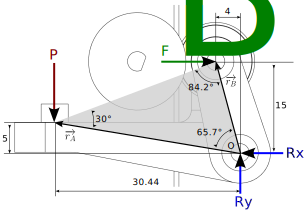
\includegraphics[width=0.8\textwidth]{forces-arm}
    \caption{Forces in actuator arm}
    \label{fig:forces-arm}
\end{figure}

The pressure or grip on the rod by the actuator is provided by the bearing and the actuator arm. The static model of the actuator arm is shown in Figure \ref{fig:forces-arm}. The sum of forces is found in Equation \ref{eq:sum-forces}, and the sum of moments at point $O$ is given in Equation \ref{eq:sum-momentums}. The force $P$ is exerted by the spring, as described by Equation \ref{eq:force-p}, where $k$ is the spring constant and $\Delta y$ is the compression. At the pin $O$, the components of the reaction force, $R_x$ and $R_y$, are present. From Equation \ref{eq:sum-momentums}, the reaction force $F_B$ at the bearing can be determined, as shown in Equation \ref{eq:force-fb}.

\begin{align}
    \label{eq:sum-forces}
    \sum \myvec{F}=0 \quad\therefore& \quad \myvec{P} + \myvec{R_y} + \myvec{F_B}+\myvec{R_x} = 0 \\
    \label{eq:sum-momentums}
    \sum \myvec{M_O}=0 \quad\therefore& \quad \myvec{r_A}\times\myvec{P} + \myvec{r_B}\times\myvec{F_B} = 0
\end{align}
\begin{equation}
    \label{eq:force-p}
    P=-k\Delta y
\end{equation}
\begin{equation}
    \label{eq:force-fb}
    F_B = \frac{r_{A,x}}{r_{B,y}}P = \frac{30.44}{15}P=-2.0293k\Delta y
\end{equation}

\begin{figure}[H]
    \centering
    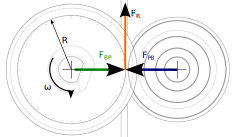
\includegraphics[width=0.7\textwidth]{friction-force}
    \caption{Friction force in rod}
    \label{fig:friction-force}
\end{figure}

The force of friction on the rod can be calculated from the force $F_B$, as illustrated in Figure \ref{fig:friction-force} and demonstrated by Equation \ref{eq:force-fr}. However, these formulas were not subjected to a comprehensive analysis because because the static friction factor, represented by the symbol $\mu_s$, were not measured. Instead, geometric constraints were of greater importance. Therefore, the spring was selected by empirically testing those with the appropriate stiffness. The drive pulley, with radius $R$, rotates at speed of $\omega$. Considering the motor's RPM, the actuator's speed specifications are provided in Table \ref{tab:actuator-specs}.

\begin{equation}
    \label{eq:force-fbp}
    F_{BP}=F_B
\end{equation}
\begin{equation}
    \label{eq:force-fr}
    F_{R}=\mu_{s}F_{BP}=-2.0293\mu_{s}k\Delta y
\end{equation}

\begin{table}[H]
    \centering
    \caption{Actuator specification}
    \label{tab:actuator-specs}
    \begin{tabular}{ll}
    \toprule
    Property & Value \\
    \midrule
    Pulley ratio ($R$) & $5.3$ mm \\
    Maximum angular velocity ($\omega_{max}$) & $7.3304$ rad/s \\
    Maximum linear velocity ($v_{max}$) & $38.85$ mm/s \\
    \bottomrule
    \end{tabular}
\end{table}